%% P--StwoS.tex
%% Sample file to use for P--S articles prepared in LaTeX
%% For two column P--S articles
%% Version1: Apr 15, 2008
%% Version2: Oct 04, 2013

%% BASIC CLASS FILE
\documentclass{pnastwo}

%% ADDITIO--L OPTIO--L STYLE FILES Font specification

%\usepackage{pnastwoF}
\usepackage{color}
%\usepackage[square,sort,comma,numbers]{natbib}


%% OPTIO--L MACRO DEFINITIONS
\def\s{\sigma}
\newcommand{\eref}[1]{(\ref{#1})}
\newcommand{\tableref}[1]{Table \ref{#1}}
\newcommand{\figref}[1]{Fig.~\ref{#1}}
\newcommand{\appref}[1]{Appendix \ref{#1}}
\newcommand{\sectionref}[1]{Section \ref{#1}}

\definecolor{Red}{RGB}{255,0,0}
\newcommand{\red}[1]{\textcolor{Red}{#1}}

%%%%%%%%%%%%
%% For P--S Only:
\url{www.pnas.org/cgi/doi/10.1073/pnas.0709640104}
\copyrightyear{2015}
\issuedate{Issue Date}
\volume{Volume}
\issuenumber{Issue Number}
%\setcounter{page}{2687} %Set page number here if desired
%%%%%%%%%%%%

\begin{document}

\title{Subjectivity predicts adjective ordering preferences}

\author{Gregory Scontras\affil{1}{Department of Psychology, Stanford University, Stanford, CA 94305},
Judith Degen\affil{1}{},
\and
Noah D.\ Goodman\affil{1}{}}

\contributor{Submitted to Proceedings of the National Academy of Sciences
of the United States of America}

%%%Newly updated.
%%% If significance statement need, then can use the below command otherwise just delete it.
\significancetext{Speakers exhibit robust ordering preferences when it comes to modification involving more than one adjective. We present experimental and corpus results showing that these preferences track the subjectivity of the adjectives at play such that less subjective adjectives occur closer to the nouns they modify. Rather than representing these preferences a fully specified ranking according to semantic classes, we show that ordering preferences more likely emerge from a desire to place more informative, less subjective content closer to the substanstive head of a nominal construction (i.e., closer to the modified noun).}

\maketitle

\begin{article}
\begin{abstract}
{Abstract here\ldots}
\end{abstract}

\keywords{language | ordering preferences | subjectivity | faultless disagreement}

%\abbreviations{SAM, self-assembled monolayer; OTS, octadecyltrichlorosilane}

\dropcap{L}inguistic competence encompasses a broad swath of information that determines the language we speak. The information, grammar, is ``mentalistic'' \cite{chomsky1965}; we observe it through the regularities in behavior of speakers and speech communities. Here we take up one such regularity, adjective ordering preferences, which determines the relative order of prenominal adjectives when more than one is used to modify a noun. The topic has received considerable attention throughout the history of generative grammar XXX and cognitive psychology XXX, owing to its remarkable stability within and across languages. Something so robust, the reasoning goes, must evidence a deep principle of the cognitive architecture that shapes language. Yet while descriptions of the phenomenon abound, an explanation continues to prove elusive. The current work serves not to solve this problem, but rather to focus attention on what we believe to be the main determinant of these preferences: adjective subjectivity. We begin with a summary of the phenomenon of interest.

\section{Background}
Speakers exhibit strong preferences when two or more adjectives are used to modify a noun, as in ``the big blue box'' or ``the good smooth purple plastic chair.'' Deviate from the preferred order, and somethings feels particularly unwieldy about ``the blue big box,'' even more so with ``the plastic good purple smooth chair.'' Indeed, for any string of pre-nominal adjectives, chances are their order is non-arbitrary. Linguists have been aware of adjective ordering preferences (or restrictions; often abbreviated ``AOR'') for well over a century now \cite{sweet1898,bloomfield1933}. Even more curious than their robustly attested status in English is their cross-linguistic regularity, observed in languages as far-flung as Celtic \cite{sproatshih1991} and Indonesian \cite{martin1969competence}.
\subsection{Psychology}
The descriptions of these preferences that have so far been proffered are nearly as diverse as the principles to which they appeal (see \cite{wulff2003} for a review of the many potential factors contributing to adjective order in production). \cite{sweet1898} proposed two principles: that adjectives which are more closely connected with the noun in meaning occur more closely to the noun, and that adjectives with a more specialized meaning occur closer to the noun. \cite{ziff1960} proposed two others: that adjectives with a less context-dependent meaning occur more closely to the noun, and that adjectives that felicitously describe a narrower set of nouns occur more closely to the noun. \cite{martin1969determinants} expands on the proposal from \cite{ziff1960}, using behavioral experiments to demonstrate that adjective order depends on adjective ``definiteness'' (i.e., context-dependence) and ``absoluteness,'' a correlate of definiteness operationalized by the number of comparisons needed to judge whether an object holds the specified property (see also \cite{kemmereretal2009} XXX).
While researchers may disagree about its details, the psychological explorations of ordering preferences converge on the idea that aspects of  adjectives' meaning (i.e., specificity, context-sensitivity, reliance on comparison, etc.) determine their relative order.

In an attempt to relate the relevant aspects of adjective meaning with the observed ordering preferences, Martin \cite{martin1969competence,martin1969determinants} proposes a specific model of language production under which more accessible adjectives are accessed earlier, and derivations are built outward from the noun. In other words, more accessible adjectives occur closer to the nouns that they modify. Crucial to this model is the hypothesis that less context-dependent adjectives and adjectives that are less sensitive to comparison are more accessible during production. When accessibility is not obeyed, non-canonical orderings occur with a so-called ``juncture,'' or pause, in the rhythm of the phrase, as in ``the blue, big box'' \cite{martin1970}.

While it provides a plausible link between the semantic factors at play and the planning of multi-adjective strings that determines their relative order, we see two problems with Martin's accessibility model. The first concerns the inverse planning that the model implicates, namely a bottom-up construction, rather than a linear parse. A more serious problem concerns adjective frequency: as Martin himself notes, more frequent adjectives are more likely to occur early, that is, farther from the noun they modify (see  \cite{wulff2003} for a similar finding).  But if accessibility tracks frequency and more accessible adjectives occur closer to the noun, we should find, contrary to fact, that more frequent adjectives occur later in multi-adjective strings.

Haiman \cite{haiman1985} proposes instead that adjective ordering preferences are symptomatic of a more general semiotic coding strategy called ``diagrammatic iconicity'' (i.e., non-arbitrary form-meaning mappings). This theory holds that distance relations in semantic space may be mapped onto distance relations in syntactic space, such that adjectives further from the noun in meaning occur farther from the noun syntactically. To move from a philosophical to a psychological theory, however, Haiman's proposal would require specifying just how more definite, less context-sensitive adjectives are closer in meaning to the nouns they modify. Indeed, a semiotic approach like Haiman's harkens back to Sweet's original description of the phenomenon of ordering preferences, namely that adjectives closer in meaning to the noun occur linearly closer to it \cite{sweet1898}. The question remains: in what sense are nominal and adjectival meaning comparable?

\subsection{Linguistics}
As part of a larger project mapping the syntax and semantics of adjectives, the literature on ordering preferences marks a turn away from the psychological determinants or ordering preferences, and toward an ordered typology of semantic classes of adjectives. These classes separate on the basis of the properties named by the adjectives that populate them. At the heart of this enterprise is \cite{dixon1982}, who argues that by prioritizing the study of adjective semantics, we may gain insight into properties of their syntactic distribution; one such property of that semantics is meant to inform concerns their relative order in pre-nominal strings. After surveying a wealth of languages, Dixon arrives the adjective classes (or ``types''), which he takes to be a cross-linguistic universal, together with their English ranking in \ref{dixon-order}.\footnote{XXX Some representative examples of Dixon's semantic classes: dimension (big, small), physical property (hard, heavy), speed (fast, slow), human propensity (happy, clever), age (new, young).} In multi-adjective strings, higher ranked adjectives occur farther from the modified noun.
\[
dimension > physical\ property > speed > 
\]
\be human\ propensity > age > color\label{dixon-order}\ee
While the ranking in \ref{dixon-order} is meant to characterize English preferences, Dixon notes that this ranking also surfaces in Hungarian and Telugu; and in Selepet (New Guinea), where adjectives typically occur post-nominally, the order is preserved in the reverse, such that higher ranked adjectives occur farther to the right of the modified noun (cf.~the discussion of Indonesian in \cite{martin1969competence} and of Celtic in \cite{sproatshih1991}; for discussion of these preferences in other languages, see \cite{hetzron1978,lapollahuang2004}).

Using a smaller and perhaps more transparently labeled set of semantic classes, \cite{sproatshih1991} proposed the ranking in \ref{ss-order}.
\be quality > size > shape > color > provenance\label{ss-order}\ee


On the basis of adjective class rankings as in \ref{dixon-order} and \ref{ss-order}, \cite{cinque1994} proposed a fully syntactic account of ordering preferences under which different adjective classes populate dedicated syntactic categories which inhabit specialized projections in the syntactic tree (see also \cite{scott2002}).\footnote{The class ranking Cinque uses as the basis for his syntactic proposal follows the ranking from \cite{sproatshih1991} in \ref{ss-order}: 
	\be quality > size > shape > color > nationality\label{cinque-order}\ee}
For example, color adjectives would inhabit the \textsc{Color} category, and project a Color Phrase.

\subsection{The upshot}
What, if anything, can we learn from all of these proposals?

Our approach to the investigation of ordering preferences synthesizes strategies from the psychological approach, probing the principles that underlie these preferences, and from the typological approach, using descriptive adjective classes to structure and inform our hypotheses.

\section{Corpus Counts}

We first conducted a corpus study to measure, for 26 adjectives from seven different classes discussed in the literature (size, quality, age, texture, shape, color, material), what their mean distance from the noun is in phrases with either two or three adjectives preceding the noun, e.g., ``a nice green color'' or ``some big heavy red cloaks''. We extracted all such cases from the Switchboard corpus as well as from both the written and spoken portions of the British National Corpus (see \emph{Materials and Methods} for details). Mean distance from the noun for each adjective class is shown in \figref{fig:distance}.

\begin{figure}[h]
	\centering
	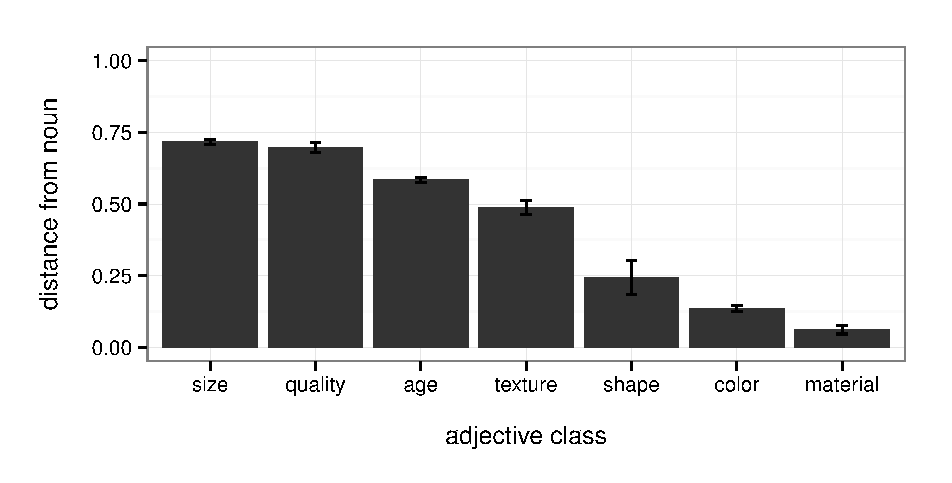
\includegraphics[width=.95\linewidth]{plots/corpus_distance_plot.eps}
	\caption{Average distance from noun by adjective class for cases with at least two modifying adjectives (39,199 cases).}\label{distance-from-noun}
	\label{fig:distance}
\end{figure}

Conducting pairwise Bonferroni-corrected comparisons between classes on the average distance-from-noun scores calculated in \figref{fig:distance} yields the following ordering preferences:

\be size \geq quality > age > texture > shape > color > material \label{inferred-order-preferences}\ee

This order \red{is identical to/closely tracks} the order previously documented \ref{REFS}.

\section{Behavioral Experiments}
	
\subsection{Subjectivity} We conducted experiment 1 to measure the subjectivity of adjectives and the broader classes to which they belong. Participants evaluated the potential for faultless disagreement between two differing descriptions of an object (\emph{Experiment 1a: Faultless Disagreement}). For example, an experimental trial might have Mary assert ``that apple is old,'' then have Bob counter with ``that apple is not old.'' To the extent that both Mary and Bob can be right in their descriptions of the apple, ``old'' admits that degree of faultless disagreement. In other words, to the extent that two people might disagree about a description without one necessarily being wrong, that description is subjective. We validated our faultless disagreement measure in a separate paradigm, which explicitly asked about the potential ``subjectivity'' of an object description like ``old apple'' (\emph{Experiment 1b: Subjectivity}). The results of these two methods are highly correlated with each other ($r^{2} = 0.89$), suggesting that the measures they invoke converge in their estimation of adjective subjectivity.

Fig.~\ref{faultless-class} plots faultless disagreement ratings for adjectives and their respective classes. Based on these aggregate scores, we infer the adjective class subjectivity raking in \ref{inferred-subjectivity} on the basis of pairwise comparisons between classes.
\be quality \geq size > texture \geq age > color \geq shape \geq material \label{inferred-subjectivity}\ee

\begin{figure}[h]
	\centering
	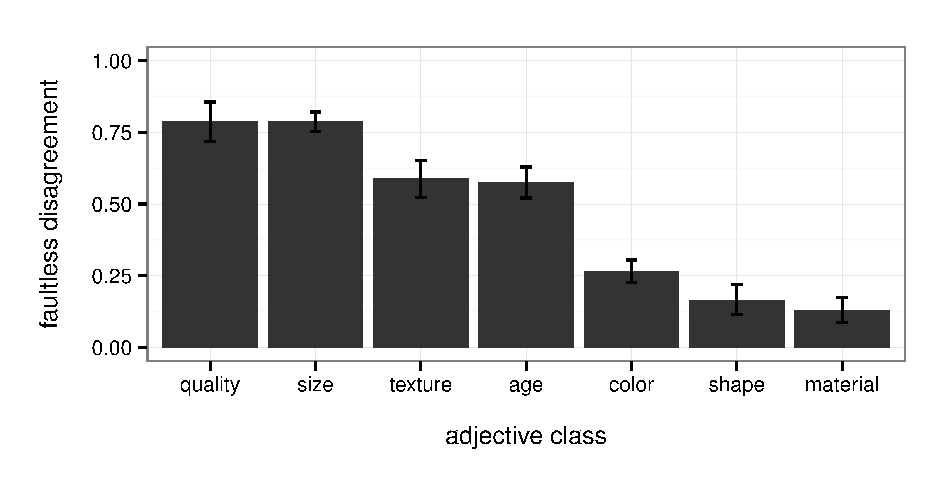
\includegraphics[width=.95\linewidth]{plots/faultless_class_plot.eps}
	\caption{Average distance from noun for each adjective class, determined by computing how often adjectives from a class occur first in preferred adjective-adjective-noun orderings.}\label{faultless-class}
\end{figure}


\subsection{Ordering preferences}
We have so far established a connection between adjective subjectivity (measured in experiment 1) and adjective proximity to nouns (obtained from corpus counts). Our next task is to verify the adjective ordering preferences that we have inferred from the corpus and from the literature on the topic, and to evaluate the predictive power of subjectivity in determining adjective order. To that end, we elicited naturalness judgments on adjective-adjective-noun object descriptions, permuting the relative order of the adjectives (\emph{Experiment 2: Ordering Preferences}). Participants indicated which ordering of an adjective-adjective-noun object description (e.g., ``the big red apple'' vs.\ ``the red big apple'') sounded more natural. 

On the basis of these naturalness ratings, we computed for each adjective-adjective pairing its preferred, canonical order. We then determined how often an adjective from a given class occurred first in an adjective-adjective-noun configuration; Fig.\ \ref{class-distance-by-adj} plots these average distance scores, where a value of 2 signals that a class's adjectives always occur first in preferred adjective-adjective-noun orderings, and a value of 1 indicates that a class's adjectives always occur second, closest to the noun.
\be size \geq quality > texture \geq age > color > shape > material \label{inferred-preference}\ee

\begin{figure}[h]
	\centering
	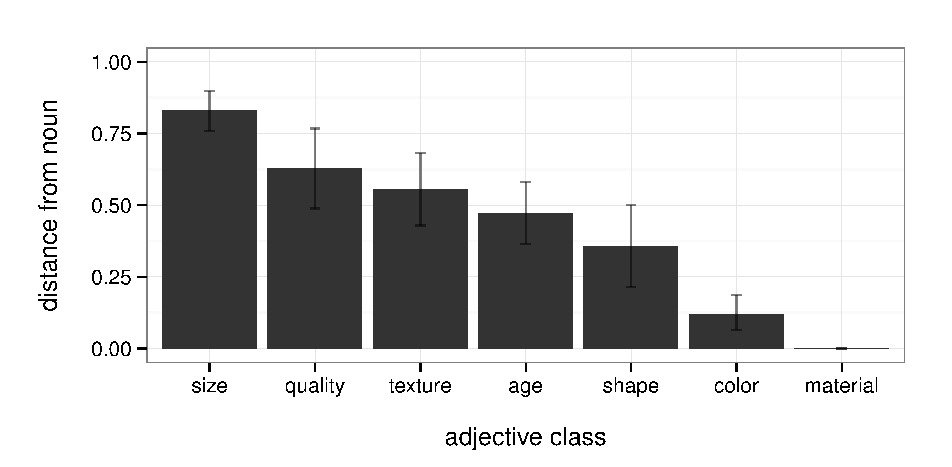
\includegraphics[width=.95\linewidth]{plots/class_distance_by_adj.eps}
	\caption{Average distance from noun for each adjective class, determined by computing how often adjectives from a class occur first in preferred adjective-adjective-noun orderings.}\label{class-distance-by-adj}
\end{figure}

Finally, and most directly related to our hypothesis concerning adjective subjectivity in ordering preferences, we compared acceptability ratings from the current experiment with faultless disagreement scores from Expt.\ 1. To do so, we first calculated a difference score for each class configuration, \textsc{class1}--\textsc{class2}, subtracting the average faultless disagreement score for \textsc{class1} from the average faultless disagreement score for \textsc{class2}. Fig.\ \ref{faultless-order} plots class configuration acceptability ratings against faultless disagreement difference scores.

\begin{figure}[h]
	\centering
	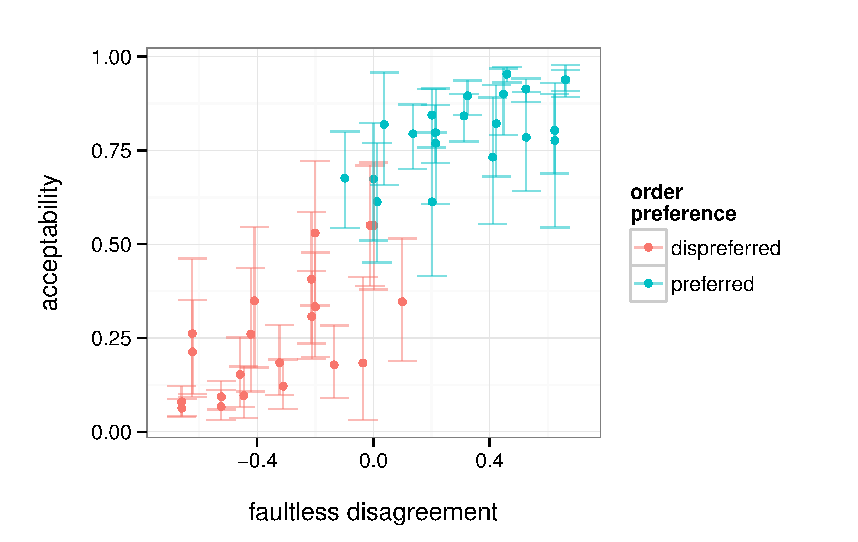
\includegraphics[width=\linewidth]{plots/faultless_order_preference.eps}
	\caption{Class-level order preferences plotted against difference in faultless disagreement between A1 and A2 (values greater than 0 indicate that the more subjective adjective class occurs farther from the noun).}\label{faultless-order}
\end{figure}






\section{Discussion}



\begin{materials}
\section{Corpus counts} 

We used TGrep2 \cite{rohde2005} and the TGrep2 Database Tools \cite{degenjaeger-tdt} to extract all ``A A N" and ``A A A N" NPs that contained one of the 26 adjectives in Table \ref{TABLREFER} from the Penn Treebank subset of the Switchboard corpus of telephone dialogs \cite{godfrey1992} as well as from the spoken and the written portions of the British National Corpus (\red{REF}). There were a total of 35,721 cases. For these cases, we computed the distance of each occurrence of our 26 target adjectives from the noun, yielding results for a total of 39,199 adjectives (180 from Switchboard, 2,232 from the spoken BNC, 36,787 from the written BNC).  See \tableref{tab:adjdist} for the distribution of cases over adjective classes.

\begin{table}
	\caption{Distribution of cases extracted from corpora over adjective classes}
	\begin{tabular}{l c c c c c c c}
	\textbf{Class} & age & size & color & quality & texture & material & shape \\
	\textbf{Count} & 15,688 & 11,576 & 5,024 & 3,790 & 1,720 & 1, 183 & 218 \\
	\textbf{Proportion} & .40 & .30 & .13 & .10 & .04 & .03 & .01
	\end{tabular}
\label{tab:adjdist}
\end{table}


For each adjective class, mean distance from the noun was computed (where position directly preceding the noun was coded as 0, the position preceding that as 1, etc.). The resulting by-class mean distances are shown in \figref{fig:distance}. To determine which differences between adjective classes are meaningful differences, we conducted Bonferroni-corrected pairwise t-tests. All differences were significant at the .0001 level except for the difference between color and shape (significant at the .04 level) and the difference between size and quality (not significant). See \tableref{tab:bonferronicorpus} for a summary. These results suggest that except for the exact position of size and quality, the order established in \figref{fig:distance} is real.

\begin{table}
\caption{Pairwise comparisons between adjective classes using t-tests with Bonferroni correction}

\begin{tabular}{l l l l l l l}
       &  age & color & material & quality & shape & size\\
color &     $<$.0001 &    --   &    --   &   -- &   --  & --\\
material &  $<$.0001 &  $<$.0001 &      --  &    -- &   -- &  --\\
quality &   $<$.0001 & $<$.0001 &         $<$.0001 &      --  &  -- &  --\\
shape &     $<$.0001 & $<$.04 &        $<$.0001 &  $<$.0001 &    -- &  --\\
size &      $<$.0001 & $<$.0001 &        $<$.0001 &  $<$.76 &    $<$.0001 &   --\\
texture &   $<$.0001 & $<$.0001 &       $<$.0001 &  $<$.0001 &    $<$.0001 &    $<$.0001
\end{tabular}
\label{tab:bonferronicorpus}
\end{table}

Pairwise comparisons using t tests with bonferroni correction
         age     color   material quality shape   size   
         color    < 2e-16 -       -        -       -       -      
         material < 2e-16 8.9e-05 -        -       -       -      
         quality  < 2e-16 < 2e-16 < 2e-16  -       -       -      
         shape    < 2e-16 0.032   1.3e-05  < 2e-16 -       -      
         size     < 2e-16 < 2e-16 < 2e-16  0.636   < 2e-16 -      
         texture  2.1e-13 < 2e-16 < 2e-16  < 2e-16 1.9e-10 < 2e-16

\section{Experiment 1a: Faultless Disagreement}
Something about our methods and how we ran the experiment


Pairwise comparisons using t tests with bonferroni correction
		         age     color   material quality shape   size   
         color    < 2e-16 -       -        -       -       -      
         material < 2e-16 0.00161 -        -       -       -      
         quality  7.6e-06 < 2e-16 < 2e-16  -       -       -      
         shape    < 2e-16 0.25546 1.00000  < 2e-16 -       -      
         size     2.8e-10 < 2e-16 < 2e-16  1.00000 < 2e-16 -      
         texture  1.00000 < 2e-16 < 2e-16  0.00011 < 2e-16 1.1e-07

\begin{table}
	\caption{Adjectives and nouns used in experimental stimuli.}
	\begin{tabular}{@{\vrule height 10.5pt depth2pt  width0pt}llllll}
	\textbf{adjective}	&	\textbf{class}	&	\textbf{adjective}	&	\textbf{class}	&	\textbf{noun}	&	\textbf{class}	\\ \hline
old	&	age	&	good	&	quality	&	apple	&	food	\\
new	&	age	&	bad	&	quality	&	banana	&	food	\\
rotten	&	age	&	round	&	shape	&	carrot	&	food	\\
fresh	&	age	&	square	&	shape	&	cheese	&	food	\\
red	&	color	&	big	&	size	&	tomato	&	food	\\
yellow	&	color	&	small	&	size	&	chair	&	furniture	\\
green	&	color	&	huge	&	size	&	couch	&	furniture	\\
blue	&	color	&	tiny	&	size	&	fan	&	furniture	\\
purple	&	color	&	short	&	size	&	TV	&	furniture	\\
brown	&	color	&	long	&	size	&	desk	&	furniture	\\
wooden	&	material	&	smooth	&	texture	\\				
plastic	&	material	&	hard	&	texture	\\				
metal	&	material	&	soft	&	texture	\\													
	\end{tabular} \label{stim-table}\caption{Adjectives and nouns used in experimental stimuli.}
\end{table}

\section{Experiment 1b: Subjectivity}

\section{Experiment 2: Ordering preferences}
We recruited 50 participants through Amazon.com's Mechanical Turk crowd-sourcing service. Participants were compensated for their participation.

Participants were asked to indicate which of two descriptions of an object sounded more natural. Each description featured a noun modified by two adjectives, for example ``the red small chair'' or ``the small red chair''. Description pairs contained the same words, with relative adjective order reversed. Descriptions were random combinations of two adjectives and a noun from the list in Table \ref{stim-table} (compiled via the procedure described in Section \ref{corpus}), with the constraint that no description contained adjectives from the same adjective class.
On each trial, participants indicated which description sounded more natural by adjusting a slider whose endpoints were labeled with the competing descriptions; an example trial appears in Fig.\ \ref{order-trial}.

\begin{figure}[h!]
	\centering
	\fbox{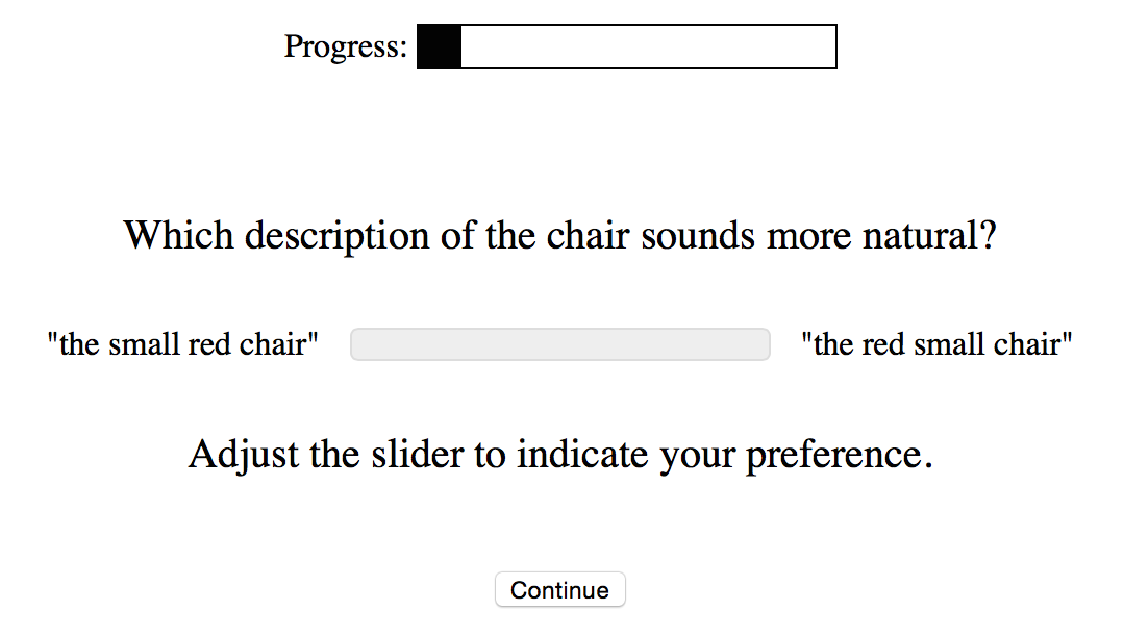
\includegraphics[width=.8\linewidth]{images/order_trial.eps}}
	\caption{Example trial from Expt.\ 1; participants indicated the more natural of two adjective-adjective-noun descriptions on a sliding scale.}\label{order-trial}
\end{figure}

Only native speakers of English with IP addresses located within the United States were included in the analyses; we analyzed data from 45 participants.



\begin{table}
	
\begin{tabular}{lllllll}
	   &    age & color & material & quality & shape & size  \\ 
color &		\textbf{$<$0.001} & -       & -        & - & - & - \\      
material &	\textbf{$<$0.001} & 1.00 & -        & - & - & - \\      
quality & 	0.98 & \textbf{$<$0.001} & \textbf{$<$0.001}  & - & - & - \\      
shape & 	1.00 & \textbf{$<$0.05} & \textbf{$<$0.001}  & \textbf{$<$0.05} & - & - \\     
size & 		\textbf{$<$0.001} & \textbf{$<$0.001} & \textbf{$<$0.001}  & 0.11 & \textbf{$<$0.001} & - \\     
texture & 	1.00 & \textbf{$<$0.001} & \textbf{$<$0.001}  & 1.00 & 0.30 & \textbf{$<$0.001}
\end{tabular}
\caption{Pairwise comparisons using t tests with Bonferroni correction \red{---would be nicer to have adjectives in the order of the plot for ease of readability; also, currently wrong numbers}}
\end{table}

\textbf{$<$0.001}



\end{materials}

\begin{acknowledgments}
This work was supported in part by Office of Naval Research Grant N000141310788 (to N.D.G.).
\end{acknowledgments}

\begin{thebibliography}{10}
	\bibitem{chomsky1965}
	N.~Chomsky, {\em Aspects of the Theory of Syntax} (1965).

	\bibitem{sweet1898}
	H.~Sweet, {\em A New English Grammar} (1898).
	
	\bibitem{bloomfield1933}
	L.~Bloomfield, {\em Language} (1933).
	
	\bibitem{sproatshih1991}
	R.~Sproat and C.~Shih, 1991. {\em The cross-linguistic distribution of adjective ordering restrictions}, Interdisciplinary approaches to language: Essays in honor of S.-Y.~Kuroda (1991), pp.~565--593.
	
	\bibitem{martin1969competence}
	J.~E.~Martin, {\em Some Competence-Process Relationships in Noun Phrases with Prenominal and Postnominal Adjectives}, Journal of Verbal Learning and Verbal Behavior, 8 (1969), pp.~471--480. 	
	
	\bibitem{wulff2003}
	S.~Wulff, {\em A multifactorial corpus analysis of adjective order in English},
	International Journal of Corpus Linguistics, 8 (2003), pp.~245‒-282.
	
	\bibitem{ziff1960}
	P.~Ziff, {\em Semantic Analysis} (1960).
	
	\bibitem{martin1969determinants}
	J.~E.~Martin, {\em Semantic Determinants of Preferred Adjective Order}, Journal of Verbal Learning and Verbal Behavior, 8 (1969), pp.~697--704. 
	
	\bibitem{martin1970}
	J.~E.~Martin, {\em Adjective Order and Juncture}, Journal of Verbal Learning and Verbal Behavior, 9 (1970), pp.~379--383. 
	
	\bibitem{haiman1985}
	J.~Haiman, {\em Natural Syntax} (1985).
	
	\bibitem{dixon1982}	
	R.~M.W.~Dixon, {\em Where have all the adjectives gone?, and other essays in semantics and syntax} (1982).
	
	\bibitem{cinque1994}
	G.~Cinque, {\em On the evidence for patial N-movement in the Romance DP}, Paths towards Universal Grammar. Studies in honor of Richard S.~Kayne (1994), pp.~85--110.
	
	\bibitem{scott2002}
	G.-J.~Scott, {\em Stacked adjectival modification and the structure of nominal phrases}, The Cartography of Syntactic Structures (2002), pp.~91--120.
	
	\bibitem{rohde2005}
	D.~Rohde, TGrep2 User Manual (2005).
	
	\bibitem{degenjaeger-tdt}
	J.~Degen and T.F.~Jaeger, The TGrep2 Database Tools (2011).
	
	\bibitem{godfrey1992}
	J.~Godfrey and E.~Holliman and J.~McDaniel, {\em Switchboard: A Telephone Speech Corpus for Research and Development}, Proceedings of ICASSP-92 (1994),
	pp.~517--520.
\end{thebibliography}


\end{article}

\end{document}






We then compared these naturalness judgments with the subjectivity scores.

For each pair of adjective classes, we determine the preferred ordering on the basis of the ratio of ratings for the each order. Ratio scores greater than 1 indicate the preferred ordering; these ratio scores for the preferred orderings are plotted in Fig.\ \ref{order-ratio}.

\begin{figure}[h]
	\centering
	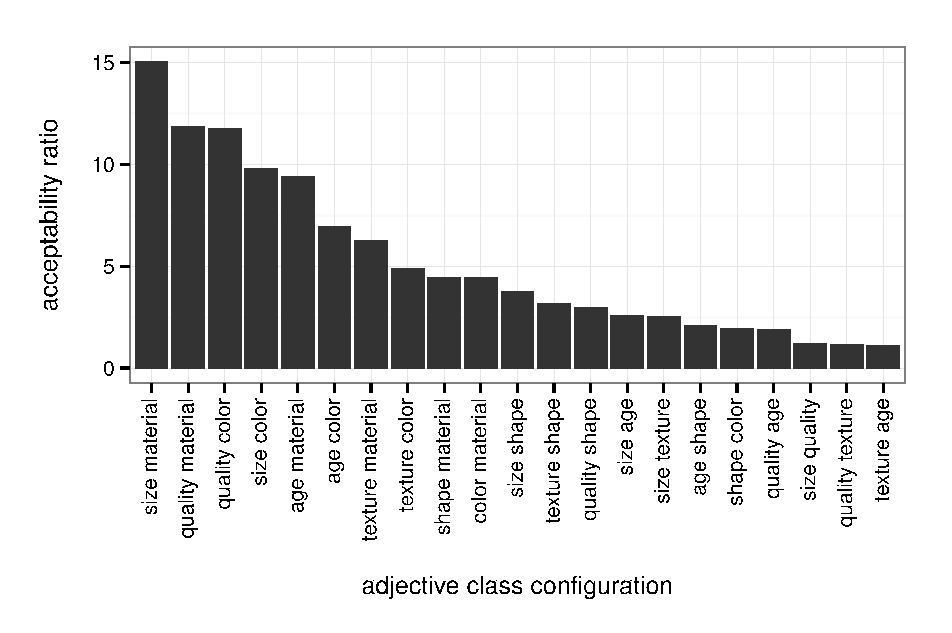
\includegraphics[width=.95\linewidth]{plots/order_ratio.eps}
	\caption{Accpetability ratios for the preferred adjective class orderings.}\label{order-ratio}
\end{figure}

On the basis of these preferred orderings, we may calculate the average distance from noun for each class, plotted in Fig.\ \ref{class-distance}. Comparing Fig.\ \ref{class-distance} with the corpus-based distance scores reported in Fig.\ \ref{distance-from-noun} confirms the reliability of the current paradigm: we replicate near exactly the qualitative order of adjective class distance from noun. 

\begin{figure}[h]
	\centering
	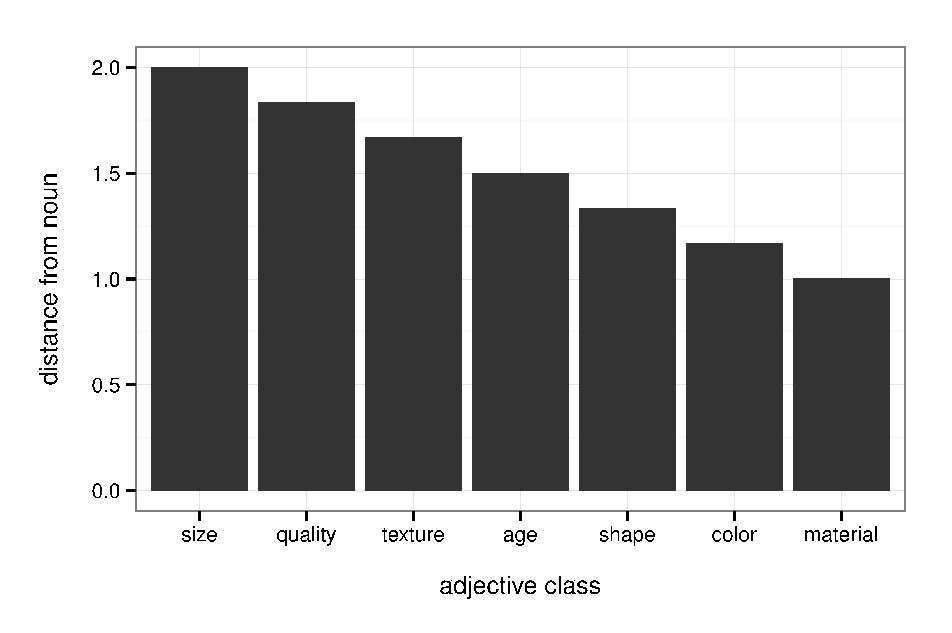
\includegraphics[width=.95\linewidth]{plots/class_distance.eps}
	\caption{Average distance from noun for each adjective class calculated from order preference ratings.}\label{class-distance}
\end{figure}

We may infer the order preferences in \ref{expt-inferred-order-preferences} (cf.\ the preferences inferred from corpus counts in \ref{inferred-order-preferences} above).
\be
size > quality > age > texture > shape > color > material\label{expt-inferred-order-preferences}\ee 
